\documentclass[9pt,twocolumn,twoside]{pnas-new}
% Use the lineno option to display guide line numbers if required.
% Note that the use of elements such as single-column equations
% may affect the guide line number alignment.

% the follow ing causes latex to not wait interactively
\nonstopmode

\setboolean{displaywatermark}{false}

\templatetype{pnasresearcharticle} % Choose template 
% {pnasresearcharticle} = Template for a two-column research article
% {pnasmathematics} = Template for a one-column mathematics article
% {pnasinvited} = Template for a PNAS invited submission

\title{Dynein walks like an Imperial AT-ST}

% Use letters for affiliations, numbers to show equal authorship (if applicable) and to indicate the corresponding author
\author[a,c,1]{Author One}

\affil[a]{Oregon State University}

% Please give the surname of the lead author for the running footer
\leadauthor{Lead author last name} 

% Please include corresponding author, author contribution and author declaration information
\authorcontributions{Please provide details of author contributions here.}
\authordeclaration{Please declare any conflict of interest here.}
\equalauthors{\textsuperscript{1}A.O.(Author One) and A.T. (Author Two) contributed equally to this work (remove if not applicable).}
\correspondingauthor{\textsuperscript{2}To whom correspondence should be addressed. E-mail: author.two\@email.com}

% Keywords are not mandatory, but authors are strongly encouraged to provide them. If provided, please include two to five keywords, separated by the pipe symbol, e.g:
\keywords{dynein $|$ Brownian dynamics $|$ powerstroke $|$ modeling} 

\begin{abstract}
Please provide an abstract of no more than 250 words in a single paragraph. Abstracts should explain to the general reader the major contributions of the article. References in the abstract must be cited in full within the abstract itself and cited in the text.
\end{abstract}

\dates{This manuscript was compiled on \today}
\doi{\url{www.pnas.org/cgi/doi/10.1073/pnas.XXXXXXXXXX}}

\newcommand\cb{0.1}
\newcommand\cm{1.5}
\newcommand\crashmovie{0}
\newcommand\ct{0.6}
\newcommand\dt{10^{-10}}
\newcommand\eqb{120}
\newcommand\eqmpost{224}
\newcommand\eqmpre{200}
\newcommand\eqt{0}
\newcommand\expunbindingconstant{0}
\newcommand\framerate{1}
\newcommand\kb{10^{8}}
\newcommand\kub{100}
\newcommand\runlabel{paperstatichisto_4}
\newcommand\ls{10.49}
\newcommand\lt{23.8}
\newcommand\nomovie{1}
\newcommand\runtime{5}
\newcommand\seed{4}


\begin{document}

% Optional adjustment to line up main text (after abstract) of first page with line numbers, when using both lineno and twocolumn options.
% You should only change this length when you've finalised the article contents.
\verticaladjustment{-2pt}

\maketitle
\thispagestyle{firststyle}
\ifthenelse{\boolean{shortarticle}}{\ifthenelse{\boolean{singlecolumn}}{\abscontentformatted}{\abscontent}}{}

\dropcap{D}ynein is a motor protein used to generate directed force in cells. The protein is a homodimer which binds to cellular filaments known as microtubules (MTs). Each monomer has several ATPase domains arranged in a larger globular domain known as the ``head''. This head is the site which hydrolyzes ATP and undergoes the conformational changes responsible for dynein's step. The head is attached via a long chain to the microtubule binding domain (MTBD). Dynein is an interesting structure in that it manages to coordinate ATPase chemistry at its head with MT-releasing chemistry at its MTBD, some 20nm away \cite{mt-atp-coupling}. The head has a long tail domain coming off it, which eventually dimerizes to the other monomer.\\

Dynein is unique in that it has a widely varied step size. Dynein's average step is 8 \textit{nm} in the forwards direction, but it is capable of taking 32 \textit{nm} steps in the forwards and reverse directions \cite{weihongpaper} \cite{yildizpaper}. This stochastic, varied stepping is contrasted with the much more regular 8 \textit{nm} step size of kinesin, another bipedal motor protein \cite{kinesin-step-size}. It has been suggested that the long separation between dynein's MTBD and dimerization sites facilitates larger diffusive searches, allowing dynein to take larger steps than kinesin \cite{cargotransport}.\\

A simple explanation for dynein's stepping pattern can be given based on only a few facts about the protein. It is known that on treatment with ATP, the tail-head-MTBD angle of a dynein monomer alters, moving the MTBD closer to the tail \cite{carteradpprimed} \cite{burgess-paper}. It is also known that the nucleotide state of the head communicates with the MTBD. ATP binding at a head ATPase shifts the MTBD from a strong to weak MT-bound state. And vice-versa, whether the MTBD is bound or unbound from the MT changes the ATPase rate at the head. From this it is possible to infer a simple model for the dynein stepping cycle. This model, known as the mechanochemical cycle \cite{cianfroccoreview}, has dynein unbind MT, kick forward, diffuse to the next MT binding site, rebind MT, then repeat. Whether a model this simple can explain dynein's behavior needs to be tested.\\

There are many relevant details about dynein which this simple model doesn't account for. Dynein is known to have low interhead communication at low separation, but to have a tension-gated stepping pattern at high separations \cite{yildizpaper}. It is also suggested that dynein's MTBD doesn't conduct an undirected search for its next MT binding site, but rather is guided by long-range electrostatic interactions from each MT binding site \cite{longrangemt}. Dynein has several cofactors which alter its dynamics. For example, the motor's stall force is tripled when exposed to dynactin and Bic2D \cite{yildizdynactin}. This is odd, since the dynactin- and Bic2D-binding site on dynein is on the tail, far from the motor heads. Many of these details suggest a complicated picture of dynein motility than a simple forward kick and pull mechanism.\\

Several computational models have been created to explain dynein's motility. \textit{Imamula et. al.} define a chemical transition model which defines all the MT- and nucleotide-bound states dynein goes through as it walks \cite{imamulamodel}. \textit{Sarlah et. al} simulate a model obeying rate constants from \textit{Imamula}, and replicate dynein's stepping trajectory \cite{sarlahmodel}. \textit{Zheng} uses normal mode analysis to simulate the dynein motor's transition from pre to post-powerstroke \cite{normalmodes}. To our knowledge, no computational model exists which takes into account the microscopic dynamics of protein-water interactions to test whether diffusion is enough for dynein motility. Here we show how a simple Brownian dynamics model can be used to test the mechanochemical cycle picture of dynein processivity.\\

\section{Results}

\begin{figure}
\centering
\includegraphics[width=\linewidth]{../../plots/time-vs-length-multiple-seeds}
\caption{Histogram of duration and length of steps taken by model.}
\label{fig:duration-length}
\end{figure}

Figure~\ref{fig:duration-length} shows the frequency of steps with
various combination of step length and step time.  We can see that...

\begin{figure}%[tbhp]
\centering
\includegraphics[width=\linewidth]{../../plots/paper-trajectory-plot.pdf}
\caption{Placeholder image of a frog with a long example caption to show justification setting.}
\label{fig:trajectory}
\end{figure}

\begin{figure}%[tbhp]
\centering
\includegraphics[width=\linewidth]{../../plots/stepping_length_histogram_paper.pdf}
\caption{Histogram of size of steps taken by model.}
\label{fig:lengthhist}
\end{figure}

\begin{figure}%[tbhp]
\centering
\includegraphics[width=\linewidth]{../../plots/stepping_time_histogram_paper.pdf}
\caption{Histogram of duration of steps taken by model.}
\label{fig:timehist}
\end{figure}

\begin{figure}%[tbhp]
\centering
\includegraphics[width=\linewidth]{../../plots/stepping_analysis_paper.pdf}
\caption{Histogram of duration of steps taken by model.}
\label{fig:timehist}
\end{figure}



\begin{table}%[tbhp]
\centering
\caption{Parameters used in model simulation.}
\begin{tabular}{lrrr}
Parameter & Model & Experimental & Source \\
\midrule
$c_b$ & $\cm \Delta G_{ATP}$ &  & \\
$c_m$ & $\cb \Delta G_{ATP}$ &  & \\
$c_t$ & $\ct \Delta G_{ATP}$ &  & \\
$k_b$ & $\kb s^{-1}$&  & \\
$k_{ub}$ & $\kub s^{-1}$ & 2.0 & \\
$L_s$ & $\ls nm$ & \cite{nativestructure} & \\
$L_t$ & $\lt nm$ & \cite{nativestructure} & \\
$\theta_b$ & $\eqb$ &  & \\
$\theta_m^{\mbox{pre}}$ & $\eqmpre$ &  & \\
$\theta_m^{\mbox{post}}$ & $\eqmpost$ &  & \\
$\theta_t$ & $\eqt$ &  & \\

\bottomrule
\end{tabular}

%% \addtabletext{nomenclature for the TSs refers to the numbered species in the table.}
\end{table}

\begin{figure}%[tbhp]
  \centering
   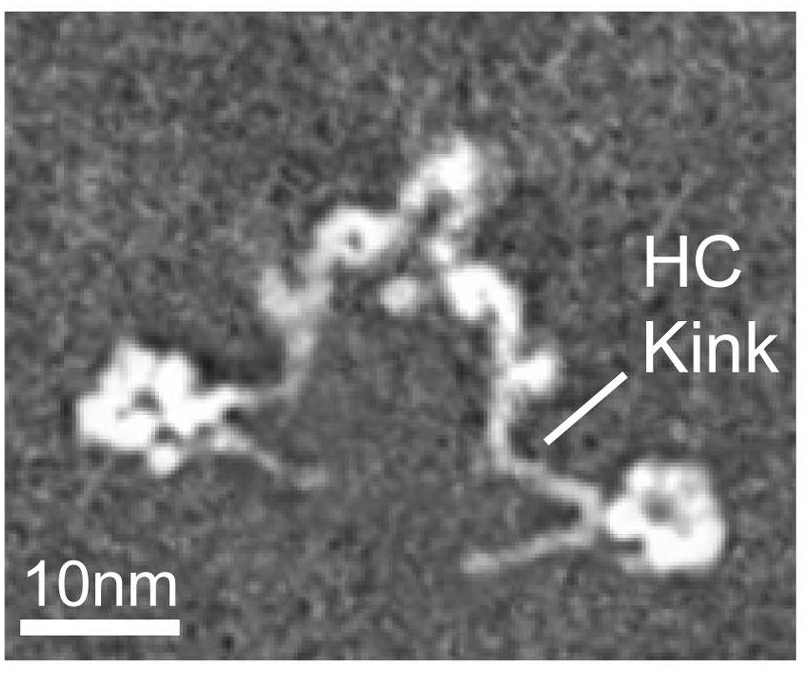
\includegraphics[width=0.3\columnwidth]{figures/schematic-1-cryoem}
   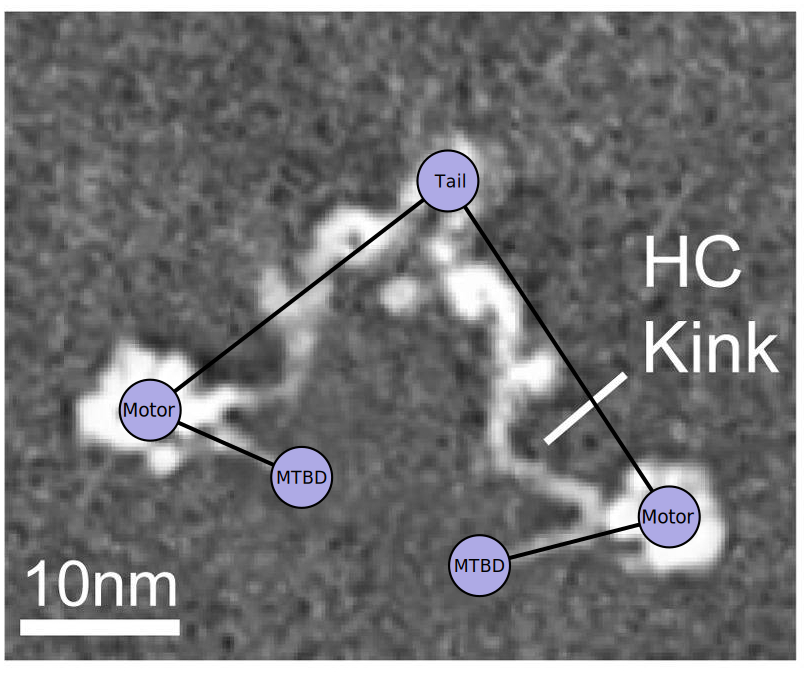
\includegraphics[width=0.3\columnwidth]{figures/schematic-1-superimposed}
   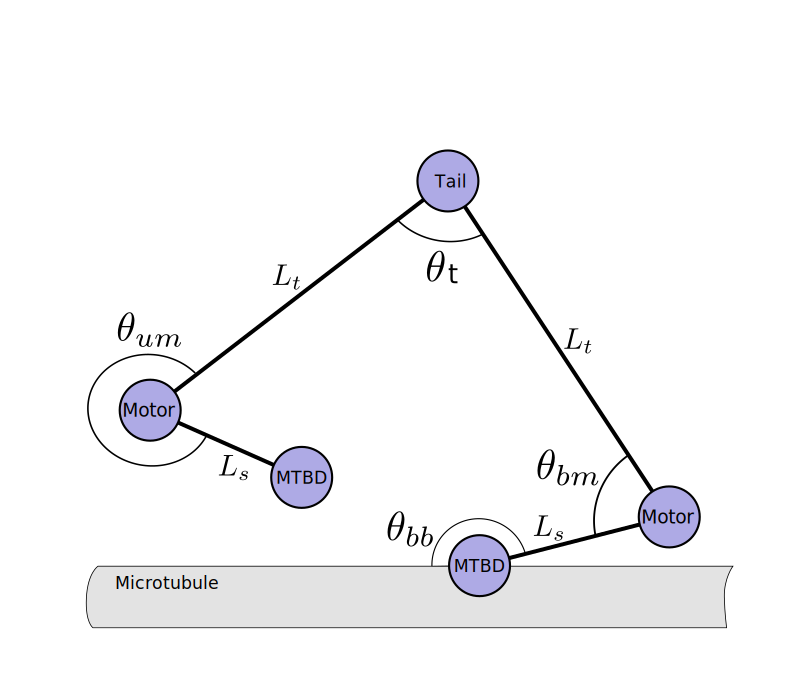
\includegraphics[width=0.3\columnwidth]{figures/schematic-1-model}

   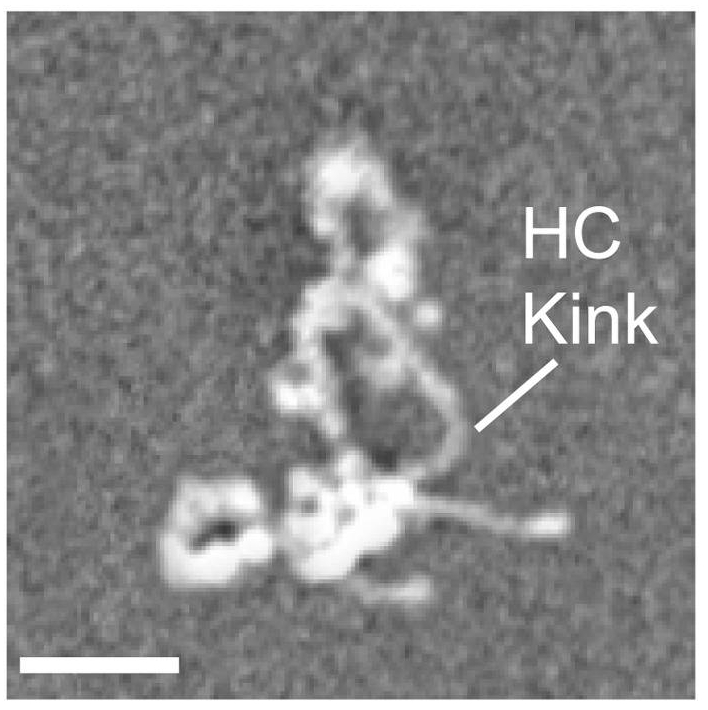
\includegraphics[width=0.3\columnwidth]{figures/schematic-2-cryoem}
   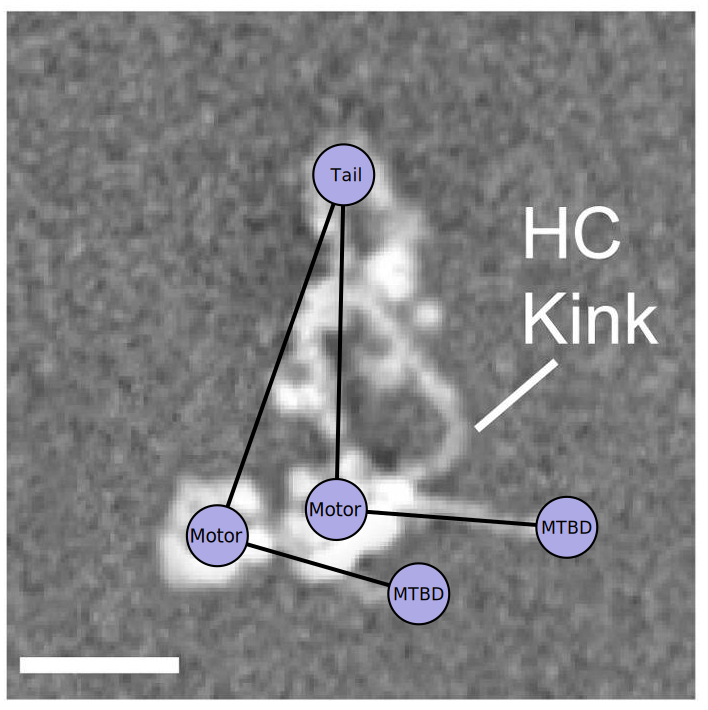
\includegraphics[width=0.3\columnwidth]{figures/schematic-2-superimposed}
   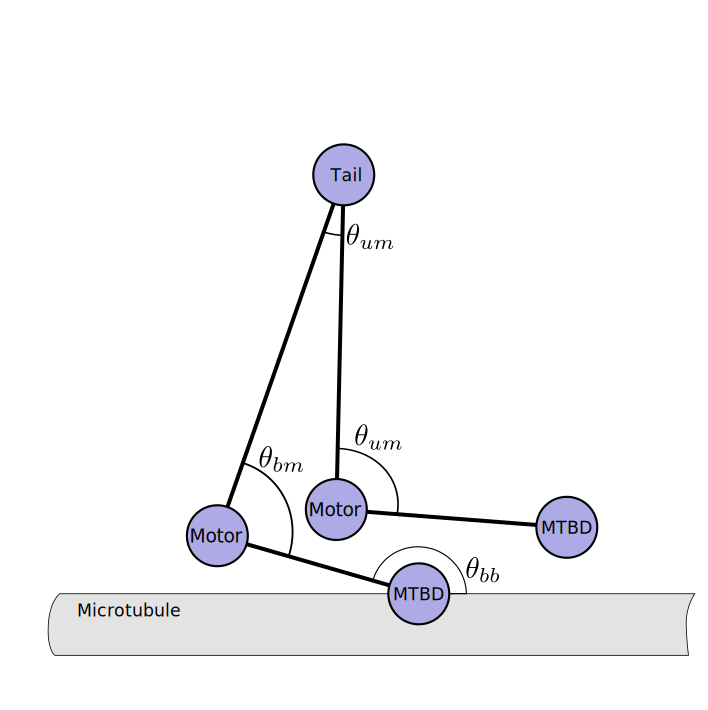
\includegraphics[width=0.3\columnwidth]{figures/schematic-2-model}
   \caption{\textbf{Model schematic superimposed on cryo-EM images of
       native dynein.} Native cryo-EM images of the full dimerized
     dynein complex composed of light, intermediate and heavy chains,
     from \cite{nativestructure}. Model schematics are superimposed
     for illustrative purpose; shown angles to not represent expected
     \textit{in vivo} equilibria. Schematics are shown docked to a
     microtubule for illustrative purposes.}
   \label{fig:modelparams}
\end{figure}

\begin{figure}%[tbhp]
  \centering
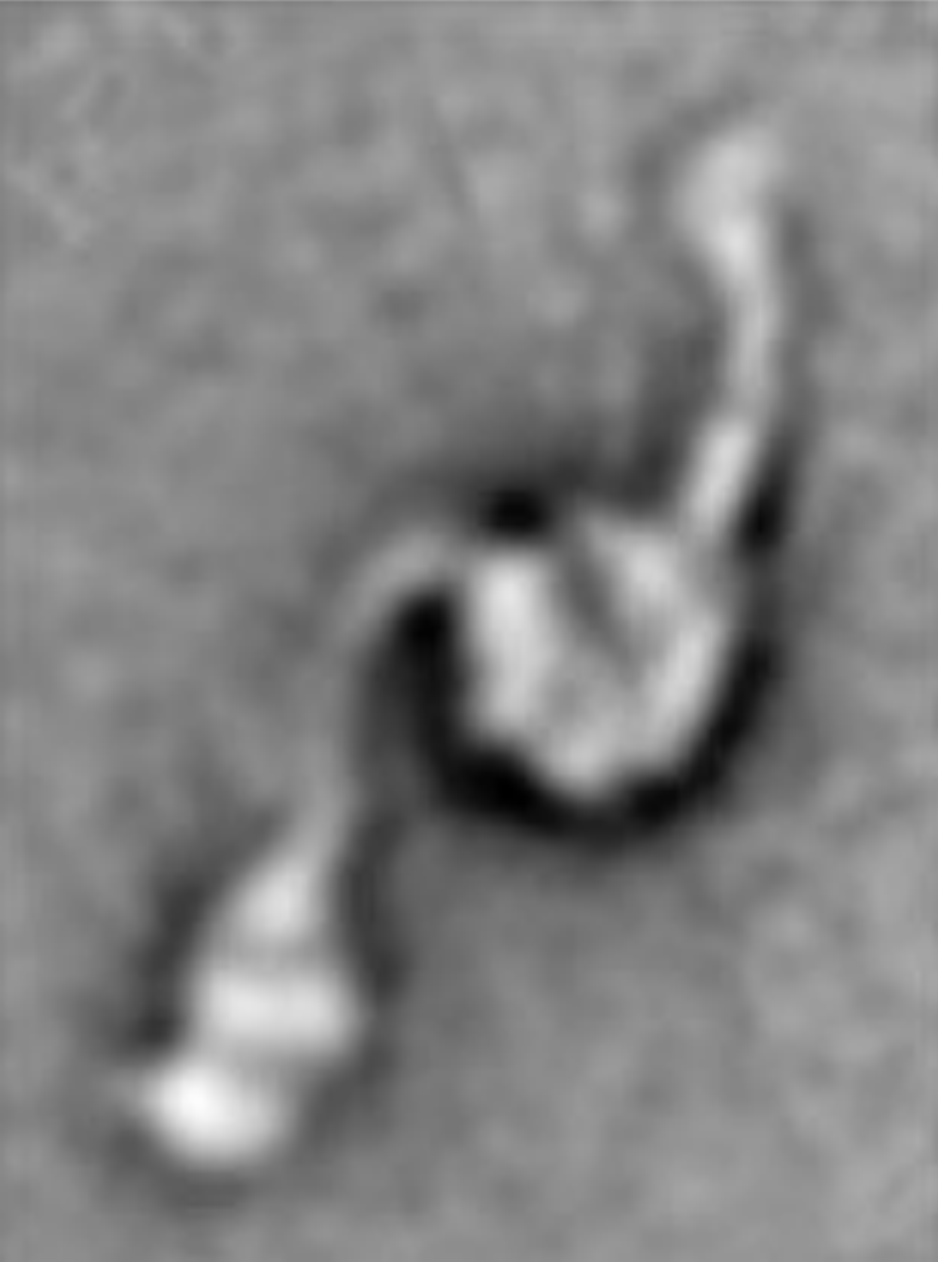
\includegraphics[width=0.5\columnwidth]{figures/schematic-prestroke}%
\includegraphics[width=0.5\columnwidth]{figures/schematic-poststroke}\\
\includegraphics[width=0.5\columnwidth]{figures/schematic-binding-angle}%
\includegraphics[width=0.5\columnwidth]{figures/schematic-full}
  \caption{\textbf{Schematic of model equilibrium angles over cryo-EM
      images.} \textbf{a.)} Prestroke and \textbf{b.)} poststroke
    dynein heavy chains superimposed with model motor angles, both
    from \cite{burgess-paper}. \textbf{c.)} Axonemal dynein bound to
    MT with model binding angle superimposed, from
    \cite{leschziner}. \textbf{d.} Full native dynein cryo-EM image
    bound to an MT with model superimposed, from
    \textbf{nativestructure}.}
\label{fig:modelangles}
\end{figure}

% \pnasbreak splits and balances the columns before the references.
% If you see unexpected formatting errors, try commenting out this line
% as it can run into problems with floats and footnotes on the final page.
\pnasbreak

\bibliography{paper}

\end{document}
